\section[Untermannigfaltigkeiten, Lagrange-Multiplikatoren]{Homöomorphismen, Untermannigfaltigkeiten und Lagrange-Multiplikatoren}
\Einleitung{Nachdem wir uns zuletzt mit stetig differenzierbaren Abbildungen mit einer stetig differenzierbaren Umkehrabbildung, den Diffeomorphismen, beschäftigt haben, werden wir nun etwas allgemeiner und untersuchen den Rang von Abbildungen.\\
Die Eigenschaft eines konstanten Rangs einer Abbildung $f:U\to\mathbb{R}^n$ ($U\subseteq\mathbb{R}^m$) werden wir nutzen, um zu zeigen, dass die Urbilder von $\qvec\in f(U)$ eine sog. \textit{Untermannigfaltigkeit} bilden.\\
Zudem werden wir die Methodik der Lagrange-Multiplikatoren betrachten, um Extrema von Funktionen unter Nebenbedingungen zu finden.}

\subsection{Wiederholung zum Rang und Abbildungen mit konstantem Rang}
Bereits letzte Woche haben wir uns angeschaut, dass wir Abbildungen durch den Rang des Differentials charakterisieren können. Weil die Begriffe so wichtig sind, wiederholen und erweitern wir sie noch einmal:
\begin{Wiederholung}{Rang einer Abbildung}
Der Rang $\rg(f)$ einer Funktion $f:U\subseteq\mathbb{R}^m\to\mathbb{R}^n$ im Punkt $\pvec\in U$ ist durch den Rang der Jacobi-Matrix $df\big|_\pvec$\footnote{d. h. der Anzahl der linear unabhängigen Zeilen bzw. Spalten} im Punkt $\pvec$ definiert.\\
Es ist stets $\rg(f)\leq\min(n,m)$.
\end{Wiederholung}
\begin{Def}
{Abbildung von konstantem Rang}
Ist $\rg(f)=:r=const\,\forall \pvec\in U$, so nennen wir $f$ eine \red{Abbildung von konstantem Rang} $r$. 
\end{Def}
\subsubsection{Exkurs: Verknüpfung zum Rang von linearen Abbildungen}
Was hat diese Definition des Ranges nun mit unserer bekannten Definition des Ranges von linearen Abbildungen $F:V\to W$ zwischen Vektorräumen zu tun?\\
Tatsächlich ist unsere 'neue' Definition konsistent damit:\\
Sei $V=\mathbb{R}^m$, $W=\mathbb{R}^n$, so ist $dF:\mathbb{R}^m\to\mathbb{R}^n$ das Differential, das ebenfalls der darstellenden Matrix $M_{E_m}^{E_n}(F)$ der linearen Abbildung bzgl. der kanonischen Basen entspricht.\\
Es ist als ganz \textit{natürlich}, sich deren Rang anzuschauen.
\begin{Beispiel}{Der Rang einer linearen Abbildung ist konstant}
Sei $F:\mathbb{R}^2\to\mathbb{R}^3,\, (x,y)\mapsto\MatrixInline{2x-y\\3y\\-4x+16y}$ eine lineare Abbildung\footnote{denn es gilt $F(\lambda v+w)=\lambda F(v)+F(w)\quad \forall v, w\in\mathbb{R}^2,\lambda\in\mathbb{R}$.}.\\
Deren Jacobi-Matrix ist dann
\begin{equation*}
    dF_{(x,y)}=\Matrix{\grad(F_1)^T\\\grad(F_2)^T\\\grad(F_3)^T}=\Matrix{2&-1\\0&3\\-4&16}.
\end{equation*}
Dies ist aber gleichzeitig die darstellende Matrix $M(F)$ bzgl. der kanonischen Basen von $\mathbb{R}^2$ und $\mathbb{R}^3$. Da keine $x$-$y$-Abhängigkeit und zudem zwei linear unabhängige Zeilen vorliegen, hat $F$ den konstanten Rang $\rg(F)=2$.\\
Da dies der Dimension des Urbildraums entspricht, ist $F$ also eine \underline{Immersion}.
\end{Beispiel}


\subsubsection{Mehr zu Immersionen}
\begin{Wiederholung}
{Immersion}
Ist $\rg(f)=m\,\forall \pvec\in U$, d. h. die Abbildung hat den konstanten Rang der Dimension des \underline{Urbildraums}, so sagen wir, dass $f$ eine \red{Immersion} ist.\\
Das Differential $df:U\to\mathbb{R}^n$ ist dann injektiv. 
\end{Wiederholung}
\blue{Ist das \underline{Differential} in $\pvec$ injektiv\footnote{Wichtig: Mit dieser Injektivität ist die Injektivität der linearen Abbildung gemeint! Also immer, wenn wir konkrete Werte von $\pvec$ einsetzen, ist $df_\pvec$ als lineare Abbildung injektiv!}, kann man sich vorstellen, dass eine in $\pvec$ angelegte Tangente stets eine nicht verschwindende Steigung hat. $f$ selbst muss aber \red{nicht} unbedingt injektiv sein, wie wir sehen werden.}
\begin{Beispiel}
{Zur Immersion (1/3)}
Die Abbildung $f:\mathbb{R}\to\mathbb{R}^3,\,\boxed{t\mapsto\MatrixInline{e^t\\t,\\t^2}}$ ist eine Immersion, denn
\begin{equation*}
    df=\Matrix{e^t\\1\\2t}
\end{equation*}
hat $\rg(f)=1\,\forall t\in\mathbb{R}$ (eine linear unabhängige Spalte).
\begin{center}
    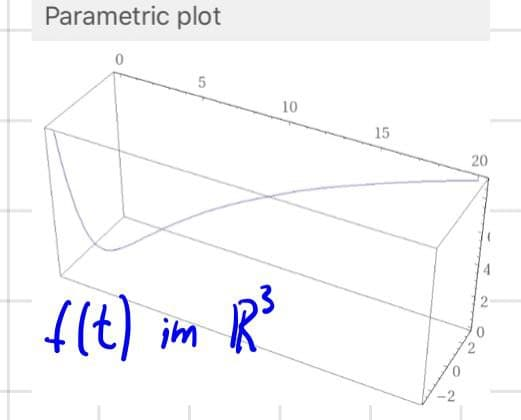
\includegraphics[width=.25\textwidth]{Dateien/10/10Immersion1.jpg}
\end{center}
\end{Beispiel}
\begin{Def}
{Kanonische Immersion}
Wir nennen\footnote{$\iota$ ist der griechische Buchstabe \textit{Iota}} für $m\leq n$ die Abbildung $\iota:\mathbb{R}^m\to\mathbb{R}^n$ mit $\iota(x_1,\ldots,x_m)=\MatrixInline{x_1\\\vdots\\x_m\\0\\\vdots\\0}$\\ (mit $n-m$ Nullzeilen) die kanonische Immersion. Deren ($n\times m$)-Ableitungsmatrix
\begin{equation*}
    d\iota=\Matrix{1&0&\cdots&0\\0&1&&\vdots\\\vdots&&\ddots&\\0&\cdots&0&1\\\vdots&&&\vdots\\0&0&\cdots&0}
\end{equation*}
hat den konstanten Rang $m$.
\end{Def}
\blue{Ein injektives Differential bedeutet aber nicht, dass auch die Abbildung selbst injektiv sein muss!}
\begin{Beispiel}
{Zur Immersion: nicht injektive Funktion (2/3)}
Die Funktion $h:\mathbb{R}\to\mathbb{R}^2,\,\boxed{h(t)=\MatrixInline{\cos(t)\\\sin(t)}}$ ist nicht injektiv, denn $h(t)=h(t+2\pi n),\,n\in\mathbb{Z}\setminus\MengeDirekt{0}$.\\
Das Differential
\begin{equation*}
    dh=\Matrix{\sin(t)\\\cos(t)}
\end{equation*}
hat aber für alle $t\in\mathbb{R}$ konstanten Rang $\rg(h)=1=\dim(\mathbb{R})$. Also ist $h$ eine Immersion.\\
Parametrischer Plot:
\begin{center}
    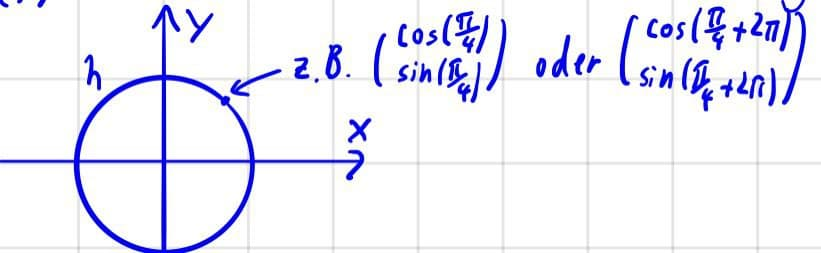
\includegraphics[width=.5\textwidth]{Dateien/10/10Immersion2.jpg}
\end{center}
\end{Beispiel}

\begin{Beispiel}
{Zur Immersion: Weitere nicht injektive Funktion (3/3)}
Die Funktion $g:\mathbb{R}\to\mathbb{R}^2,\,\boxed{g(t)=\MatrixInline{t^2-1\\t(t^2-1)}}$ ist eine Immersion, denn
\begin{equation*}
    \rg(g)=\rg(dg_t)=\rg\Matrix{2t\\t^2-1+2t^2}=1.
\end{equation*}
Das Differential ist wieder injektiv, die Funktion selbst nicht, denn $g(1)=\MatrixInline{0\\0}=g(-1)$. \Lightning
\begin{center}
    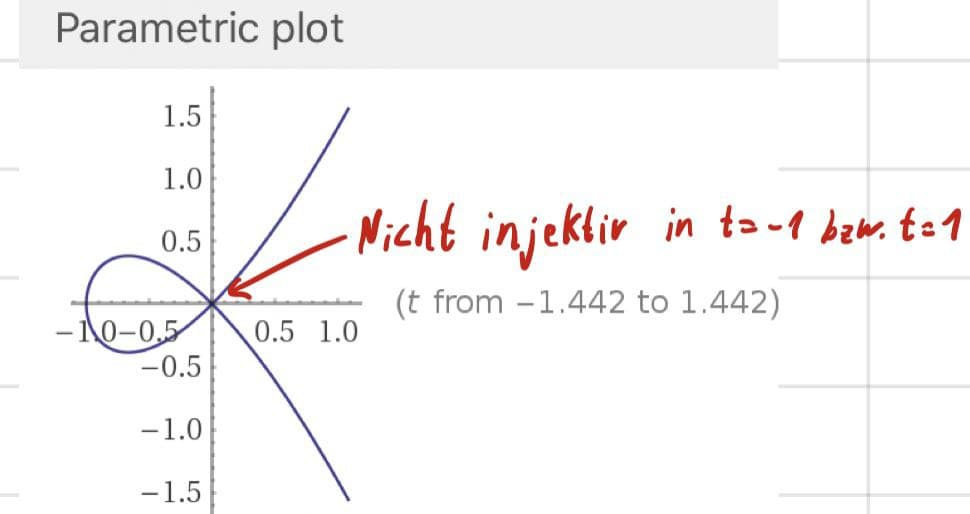
\includegraphics[width=.35\textwidth]{Dateien/10/10Immersion3.jpg}
\end{center}
\end{Beispiel}

\subsubsection{Mehr zur Submersion}
\begin{Def}
{Submersion}
Ist $\rg(f)=n\,\forall \pvec\in U$, d. h. die Abbildung hat den konstanten Rang der Dimension des \underline{Bildraumes}, so sagen wir, dass $f$ eine \red{Submersion} ist.\\
Das Differential $df:U\to\mathbb{R}^n$ ist dann surjektiv.
\end{Def}
\blue{Ist das \underline{Differential} in $\pvec$ surjektiv, kann man sich vorstellen, dass eine in $\pvec$ angelegte Tangente surjektiv ist. $f$ selbst muss aber \red{nicht} unbedingt surjektiv sein.}
\begin{Beispiel}
{Zur Submersion (1/3)}
Die Abbildung $f:\mathbb{R}^3\to\mathbb{R}^2,\,\boxed{f(x,y,z)=\MatrixInline{e^xy\\e^y+z}}$ ist eine Submersion, denn
\begin{equation*}
    df=\Matrix{e^xy&e^x&0\\0&e^y&1}
\end{equation*}
hat konstanten Rang $\rg(f)=2=\dim(\mathbb{R}^2)\,\forall x,y,z\in\mathbb{R}$, denn egal, was wir für $x,y$ und $z$ einsetzen, stets zwei linear unabhängige Zeilen haben.
\end{Beispiel}
\begin{Def}
{Kanonische Submersion}
Wir nennen für $m\geq n$ die Abbildung $\pi:\mathbb{R}^m\to\mathbb{R}^n$ mit $\pi(x_1,\ldots,x_m)=\MatrixInline{x_1\\\vdots\\x_n}$ die kanonische Submersion (alle überflüssigen Komponenten werden abgeschnitten). Deren ($n\times m$)-Jacobi-Matrix
\begin{equation*}
    d\iota=\Matrix{1&\cdots&0&\cdots&0\\\vdots&\ddots&&&\vdots\\0&\cdots&1&\cdots&0}
\end{equation*}
hat den konstanten Rang $n$.
\end{Def}
\blue{Ein surjektives Differential bedeutet nicht, dass auch die Abbildung selbst surjektiv sein muss!}
\begin{Beispiel}
{Zur Submersion: Nicht surjektive Funktion (2/3)}
Sei $g:\mathbb{R}\to\mathbb{R},\,\boxed{g(x)=e^x}$ ist nicht surjektiv\footnote{bildet ja nur auf $\mathbb{R}_+$ und nicht komplett auf $\mathbb{R}$ ab}, aber das Differential $dg=(e^x)$ hat für alle $x$ konstanten Rang 1! Hier liegt also sowohl eine Submersion als auch eine Immersion vor.
\end{Beispiel}
\blue{Andersherum müssen surjektive Abbildungen nicht unbedingt Submersionen sein!}
\begin{Beispiel}
{Zur Submersion: Surjektive Funktion{,} die keine Submersion ist (3/3)}
Wir betrachten die surjektive Funktion $j:\mathbb{R}\to\mathbb{R},\,\boxed{j(x)=x^3}$ mit $dj=(3x^2)$. Hierbei ist
\begin{equation*}
    \rg(j)=\Cases{1\quad & x\in\mathbb{R}\setminus\MengeDirekt{0}\\0&x=0}.
\end{equation*}
\blue{Hier entspricht $dj_x$ ja immer der Tangentensteigung. Diese ist 0 in $x=0$, die Tangente ist hier nicht surjektiv. Dies ist gleichzeig ein Beispiel für eine injektive Funktion, die keine Immersion ist!}
\end{Beispiel}

\subsubsection{Sätze zum Rang}
\begin{Satz}{Satz}
{Diffeomorphismen haben konstanten Rang}
Haben wir mit $f:U\to V$ ($U\subseteq\mathbb{R}^m$, $V\subseteq\mathbb{R}^n$ jeweils offen) einen Diffeomorphismus vorliegen, so ist $\boxed{\rg(f)=m=n}\,\forall x\in U$, da das Differential $\forall x\in U$ invertierbar sein muss und somit vollen Rang $\rg(df)=m=n$ hat. 
\end{Satz}
\begin{Satz}{Satz}
{Normalform für Abbildungen von konstantem Rang}
Für eine $C^k$-Abbildung\footnote{also $k$-fach stetig differenzierbar} $\textcolor{blue}{f}:\textcolor{mygreen}{U}\to\textcolor{blue}{\mathbb{R}^n}$ mit konstantem Rang $\rg(f)=\textcolor{orange}{r}$ gilt für $\textcolor{mygreen}{\pvec\in U}$:\\
Es gibt offene Umgebungen $\textcolor{mygreen}{V\subseteq U}$ von $\textcolor{mygreen}{\pvec}$, $\textcolor{blue}{W\subseteq \mathbb{R}^n}$ von $\textcolor{blue}{f(\pvec)}$ und $C^k$-Diffeomorphismen $\textcolor{mygreen}{\varphi:V\to V\subseteq\mathbb{R}^m}$ und $\textcolor{blue}{\psi:W}\to\textcolor{blue}{\psi(W)\subseteq\mathbb{R}^n}$, sodass die Verknüpfung
\begin{equation*}
    (\textcolor{blue}{\psi}\circ\textcolor{blue}{ f}\circ\textcolor{mygreen}{\varphi^{-1}})(\textcolor{mygreen}{x_1,\ldots,x_m})=(x_1,\ldots, x_{\textcolor{orange}{r}},\overbrace{0,\ldots,0}^{\textcolor{blue}{n}-\textcolor{orange}{r}})\quad\tx{für alle }\textcolor{mygreen}{\xvec\in \varphi(V)}
\end{equation*}
ist.\\
Dies ist die \red{Normalform}.\\
In der folgenden Abbildung haben wir versucht, die Abbildungskette
\begin{equation*}
    \textcolor{mygreen}{\varphi(V)}\to \textcolor{mygreen}{V}\to \textcolor{blue}{f(V)}\to\textcolor{blue}{\psi(f(V))}
\end{equation*}
darzustellen:
\begin{center}
    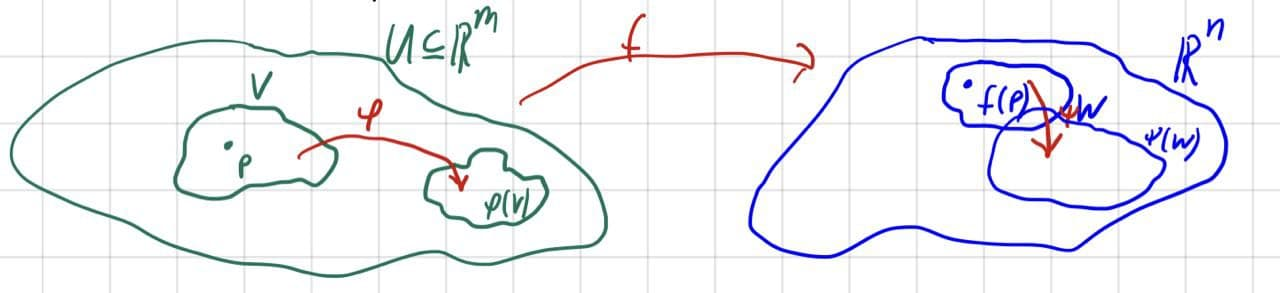
\includegraphics[width=.5\textwidth]{Dateien/10/10Normalform.jpg}
\end{center}
\end{Satz}
\blue{\textbf{Zum Verständnis dieses Satzes}:\\
Wenn die Abbildung $f$ auf $U$ den konstanten Rang $\rg(f)=\textcolor{orange}{r}$ hat, können wir um den Urbildpunkt $\textcolor{mygreen}{\pvec}$ ($m$-dimensional) und dessen Bildpunkt $\textcolor{blue}{f(\pvec)}$ ($n$-dimensional) offene Umgebungen $\textcolor{mygreen}{V\subseteq U},\textcolor{blue}{W\subseteq \mathbb{R}^n}$ und außerdem zwei $C^k$-Diffeomorphismen $\varphi$ und $\psi$ finden, sodass wir $f$ mit diesen in eine Form transformieren können, die der kanonischen Abbildung mit Rang $\textcolor{orange}{r}$ entspricht.\\
Die Diffeomorphismen $\varphi$ und $\psi$ stellen nur Koordinatentransformationen dar, die eigentliche Abbildung $\textcolor{mygreen}{U}\to\textcolor{blue}{\mathbb{R}^n}$ geschieht immer noch durch $f$.}\\
\red{Liegt mit $f$ eine Submersion oder Immersion vor, können wir uns eine dieser beiden Koordinatentransformationen sparen:}
\begin{Satz}
{Satz}{Spezialfälle der Normalformen}
Seien $U\subseteq \mathbb{R}^m$ offen, $\pvec\in U$, $f:U\to\mathbb{R}^n$ eine $C^k$-Abbildung mit $\rg(f)_p=r$.
\begin{itemize}
    \item Ist $r=n$ (und $n\leq m$), so existiert eine offene Umgebung $V\subseteq U$ des Urbilds $\pvec\in U$ und $\varphi:V\to\varphi(V)\subseteq\mathbb{R}^m$, sodass
    \begin{equation*}
        (f\circ\varphi^{-1})(x_1,\ldots,x_m)=\MatrixInline{x_1\\\vdots\\x_n}
    \end{equation*}
    auf $\varphi(V)$. Lokal ist $f$ also eine Submersion und mithilfe des Diffeomorphismus $\varphi$ auf die kanonische Submersion zurückzuführen.
    \item Ist $r=m$ (und $m\leq n$), so existiert eine offene Umgebung $W\subseteq \mathbb{R}^n$ des Bildes $f(\pvec)$ und $\psi:W\to\psi(W)\subseteq\mathbb{R}^n$, sodass
    \begin{equation*}
        (\psi\circ f)(x_1,\ldots,x_m)=\MatrixInline{x_1\\\vdots\\x_m\\0\\\vdots\\0}
    \end{equation*}
    in einer Umgebung von $\pvec$. Lokal ist $f$ also eine Immersion und mithilfe des Diffeomorphismus $\psi$ auf die kanonische Immersion zurückzuführen.
\end{itemize}
\end{Satz}
\begin{Beispiel}
{Normalform einer Submersion}
Für die vorhin betrachtete Submersion $g:\mathbb{R}\to\mathbb{R},\,g(x)=e^x$ wäre dies die Abbildung $\varphi:\mathbb{R}\to\mathbb{R}_+,\,\varphi(x)=e^x$ mit $\varphi^{-1}:\mathbb{R}_+\to\mathbb{R},\varphi^{-1}(x)=\ln(x)$, sodass $(f\circ\varphi^{-1})(x)=f(\ln(x))=e^{\ln(x)}=x$ der Normalform entspricht.
\end{Beispiel}
Auf Folie 299 ist zudem ein weiteres Beispiel zu finden.


\subsubsection{Homömorphismen}
Als Vorbereitung auf Untermannigfaltigkeiten benötigen wir zunächst noch einen weiteren Begriff, um Abbildungen zu klassifizieren:
\begin{Def}
{Homöomorphismus}
Wir nennen eine Abbildung $\phi:X\to Y$ (zwischen metrischen Räumen $X$ und $Y$) einen \red{Homöomorphismus}, wenn sie die folgenden Eigenschaften hat:
\begin{enumerate}
    \item $\phi$ ist bijektiv.
    \item $\phi$ ist stetig.
    \item $\phi$ besitzt eine stetige Umkehrabbildung $\phi^{-1}:Y\to X$.
\end{enumerate}
Wir schreiben auch $\phi:X\overset{\sim}{\to}Y$, wenn $\phi$ homöomorph von $X$ auf $Y$ abbildet.
\end{Def}
\blue{Jeder Diffeomorphismus ist somit ein Homöomorphismus, da $\mathbb{R}^n$ ein metrischer Raum und die Umkehrabbildung per Definition stetig differenzierbar und somit stetig ist.\\
Die Forderung, dass auch die Umkehrabbildung stetig sein soll, ist für metrische Räume entscheidend. In der Vorlesung habt ihr im Zusammenhang mit den topologischen Grundbegriffen folgenden Satz kennengelernt:}
\begin{Satz}
    {Satz}{Stetige Abbildungen zwischen metrischen Räumen}
    Für eine Abbildung $F:\,X\rightarrow Y$ zwischen metrischen Räumen sind die folgenden Aussagen äquivalent:
    \begin{enumerate}
        \item $F$ ist stetig
        \item Urbilder $F^{-1}(U)$ aller offenen Mengen $U\subseteq Y$ sind offen
        \item Urbilder $F^{-1}(A)$ aller abgeschlossenen Mengen $A\subseteq Y$ sind abgeschlossen
    \end{enumerate}
    Eine stetige Abbildung bildet also offene Mengen auf offene Mengen und abgeschlossene Mengen auf abgeschlossene Mengen ab!
\end{Satz}
\blue{Existiert ein Homöomorphismus $F$ zwischen zwei metrischen Räumen $X$ und $Y$ (oder allgemeiner: zwischen zwei topologischen Räumen), dann gibt es zu jeder offenen Menge $U\subseteq X$ ein offenes Pendant $F(U)\subseteq Y$ \underline{und umgekehrt}. Dasselbe gilt für abgeschlossene Mengen. \\
Sind also zwei metrische Räume homöomorph, dann bedeutet dies, dass sie \glqq{}im wesentlichen gleich sind\grqq{}, also dieselben topologischen Eigenschaften teilen.}
\begin{Beispiel}
    {Stereographische Projektion}
    Dies ist ein beliebtes und auch wichtiges Beispiel in der theoretischen Physik (zum Beispiel in der Stringtheorie)! Wir leiten sie im Folgenden ausführlich für einen Halbkreis her, für eine Kugel siehe Vorlesung.\\
    
    Ziel: wir wollen die reellen Zahlen (bis auf das Intervall $(-r,r)$) auf einen Halbkreis abbilden. Das Prinzip dazu zeigt die folgende Skizze:
    \begin{center}
        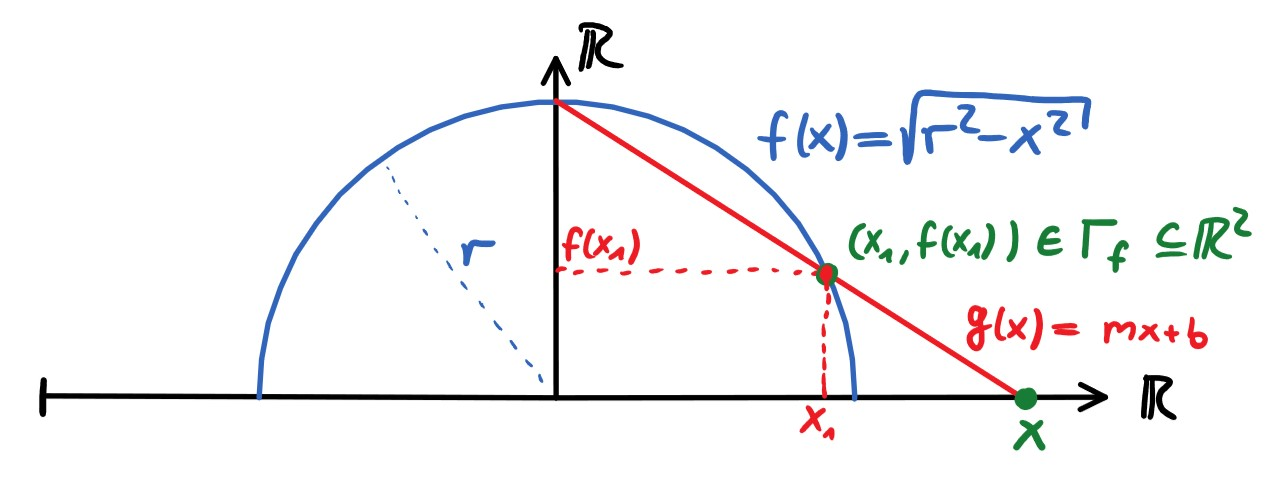
\includegraphics[width=.8\textwidth]{Dateien/10/10StereographischeProjektion.jpg}
    \end{center}
    Die stereographische Projektion ordnet jedem $x\in\mathbb{R}\setminus(-r,r)$ einen Punkt $(x_1(x), f(x_1(x)))$ gemäß der Skizze auf dem Halbkreis $f(x)=\sqrt{r^2-x^2}$ mit dem Radius $r$ zu. Wie sieht nun diese Projektionsfunktion aus? \\
    
    Zunächst stellen wir die Geradengleichung von $g(x)=mx+b$ auf:
    \begin{align*}
        m=\frac{r-f(x_1)}{0-x_1}&=-\frac{r-f(x_1)}{x_1} \qquad (b=r) \\
        \Rightarrow g(x) &= -\frac{r-f(x_1)}{x_1}x+r=-\frac{r-\sqrt{r^2-x_1^2}}{x_1}x+r.
    \end{align*}
    Nun setzen wir $g(x)=0$ und formen nach $x_1(x)$ um:
    \begin{align*}
        0=g(x)&=-\frac{r-\sqrt{r^2-x_1^2}}{x_1}x+r \quad\Leftrightarrow\quad r-\frac{x_1}{x}r=\sqrt{r^2-x_1^2} \\
        \Leftrightarrow\quad &x_1^2(1+\frac{r^2}{x^2})-2r^2\frac{x_1}{x}=0 \quad\Leftrightarrow\quad x_1^2-x_1\frac{2r^2x}{x^2+r^2}=0 \\
        \Leftrightarrow\quad &x_1(x)=\frac{2r^2x}{x^2+r^2}.
    \end{align*}
    Da $x_1\in\mathbb{R}\setminus (-r,r)$, ist $x_1=0$ keine Lösung dieser Gleichung. Wir können nun aus dieser Vorschrift eine Projektion $\varphi$ bilden, die definiert ist durch
    \begin{equation*}
        \varphi:\,\mathbb{R}\setminus(-r,r)\longrightarrow \Gamma_f, \quad \varphi(x)=(x_1(x), f(x_1(x)))
    \end{equation*}
    Zur Erinnerung: $\Gamma_f=\Menge{(x,f(x))\in\mathbb{R}^2}{x\in(-r,r)}$ (siehe Mathe 1). \\
    Einsetzen liefert:
    \begin{align*}
        \varphi(x)&=\Big( \frac{2r^2x}{x^2+r^2}, f\big( \frac{2r^2x}{x^2+r^2} \big) \Big) = \Big( \frac{2r^2x}{x^2+r^2},\sqrt{r^2-\frac{4r^4x^2}{(x^2+r^2)^2}} \Big) \\
        &= \Big( \frac{2r^2x}{x^2+r^2},r\sqrt{\frac{(x^2+r^2)^2-4r^2x^2}{(x^2+r^2)^2}} \Big) = \Big( \frac{2r^2x}{x^2+r^2},r\sqrt{\frac{x^4+r^4+2x^2r^2-4r^2x^2}{(x^2+r^2)^2}} \Big) \\
        &= \Big( \frac{2r^2x}{x^2+r^2},r\sqrt{\frac{(x^2-r^2)^2}{(x^2+r^2)^2}} \Big) = \Big( \frac{2r^2x}{x^2+r^2}, \frac{r(x^2-r^2)}{(x^2+r^2)} \Big) \\
        &=\frac{r}{x^2+r^2}\big( 2rx, x^2-r^2 \big)
    \end{align*}
    Ist dies nun ein Homöomorphismus? Dazu checken wir ab:
    \begin{itemize}
        \item Wir haben die Funktion so konstruiert, dass sie bijektiv ist
        \item Als Zusammensetzung stetiger Funktionen ist sie stetig
        \item Eine Umkehrabbildung kriegen wir (wobei $x=x_1$ und $y=f(x_1)$) wie folgt:
        \begin{align*}
            g(\varphi^{-1}(x,y))&=-\frac{r-y}{x}\varphi^{-1}(x,y)+r = 0 \qquad\, (\varphi^{-1}:\,\Gamma_f\longrightarrow \mathbb{R}\setminus(-r,r)) \\
            &\Leftrightarrow \varphi^{-1}(x,y)=\frac{rx}{r-y} \qquad \qquad \quad (y=f(x)=\sqrt{r^2-x^2})
        \end{align*}
    \end{itemize}
    Das dies wirklich eine Umkehrabbildung von $\varphi$ ist, müssen wir natürlich noch sauber prüfen. Zuerst rechnen wir
    \begin{align*}
        \varphi&(\varphi^{-1}(x,y))=\frac{r}{\frac{r^2x^2}{(r-y)^2}+r^2}\Big( 2r\frac{rx}{r-y}, \frac{r^2x^2}{(r-y)^2}-r^2 \Big) \\
        &= \Big( \frac{2rx(r-y)}{x^2+r^2+y^2-2ry}, \frac{r(x^2-r^2-y^2+2ry)}{x^2+r^2+y^2-2ry} \Big) \qquad (r^2=x^2+y^2,\, y^2=r^2-x^2) \\
        &= \Big( \frac{2rx(r-y)}{2r^2-2ry}, \frac{2ry-2y^2}{2(r-y)} \Big) = \Big( x\frac{r(r-y)}{r(r-y)}, y\frac{r-y}{r-y} \Big) = (x,y)
    \end{align*}
    und natürlich das Ganze auch nochmal in die andere Richtung
    \begin{align*}
        \varphi^{-1}(\varphi(x)) &= r\frac{2r^3x}{r^2+x^2}\Big( r-r\frac{x^2-r^2}{x^2+r^2} \Big)^{-1} = 2r^3x\big[ r(x^2+r^2)-r(x^2-r^2) \big]^{-1} = \frac{2r^3}{2r^3}x=x.
    \end{align*}
    Wir haben also wirklich eine Umkehrabbildung gefunden:
    \begin{equation*}
        \varphi^{-1}:\, \Gamma_f\rightarrow\mathbb{R}\setminus(-r,r), \varphi^{-1}(x,y)=\frac{rx}{r-y}
    \end{equation*}
    Diese Funktion setzt sich aus stetigen Funktionen zusammen und ist deswegen ebenfalls stetig. Somit ist $\varphi$ ein Homöomorphismus! \\
    
    Wir können sogar einen Schritt weitergehen und zeigen, dass $\varphi$ auch ein Diffeomorphismus ist. Dazu müssen wir einfach die Differentiale von $\varphi$ und $\varphi^{-1}$ aufstellen:
    \begin{align*}
        \text{d}\varphi_x&=\Matrix{\partial_x\varphi_1 \\ \partial_x\varphi_2} = \frac{2r^2}{(x^2+r^2)^2}\Matrix{r^2-x^2 \\ 2rx} \\
        \text{d}\varphi^{-1}&=\Matrix{\partial_x\varphi^{-1} & \partial_y \varphi^{-1}}=\Matrix{\frac{r}{r-y} & -\frac{rx}{(r-y)^2}}.
    \end{align*}
    Beide Differentiale existieren über den gesamten Definitionsbereich, womit $\varphi$
    und $\varphi^{-1}$ differenzierbar sind. Also ist $\varphi$ ein Diffeomorphismus. Abschließend können wir noch klären, ob nun wirklich d$\varphi^{-1}_x = \text{d}(\varphi^{-1})_{\varphi(x)}$ gilt (Satz auf Folie 272 im Skript):
    \begin{align*}
        \text{d}\varphi_x^{-1}&=\frac{x^2+r^2}{2r^2}\big( 1, \frac{x}{r} \big) \\
        \text{d}(\varphi^{-1})_{\varphi(x)}&=\Big( r\big(r-\frac{r(x^2-r^2)}{x^2+r^2} \big)^{-1}, -\frac{2r^3x}{x^2+r^2}\big( r-r\frac{x^2-r^2}{x^2+r^2} \big)^{-2} \Big) \\ &= \Big( \frac{x^2+r^2}{2r^2}, \frac{x(x^2+r^2)}{2r^3} \Big) = \frac{x^2+r^2}{2r^2}\big( 1, \frac{x}{r} \big),
    \end{align*}
    womit wir auch diese Zweifel ausgeräumt hätten.

\end{Beispiel}

\begin{Beispiel}
    {Beispiel für eine nicht homöomorphe Funktion}
    Die Sphäre sei gegeben durch $S^1=\Menge{z\in\mathbb{C}}{\Abs{z}=1}$. Wir betrachten nun die Funktion 
    \begin{equation*}
        \varphi:\,[0,2\pi)\rightarrow S^1, \quad \varphi(x)=e^{ix}
    \end{equation*}
    Diese Funktion ist stetig und bijektiv. Wir betrachten nun die Folge
    \begin{equation*}
        x_n := \varphi(2\pi-\frac{1}{n})=e^{i(2\pi-\frac{1}{n})}=e^{-\frac{i}{n}}
    \end{equation*}
    mit dem Grenzwert
    \begin{equation*}
        \lim_{n\rightarrow\infty} x_n = \lim_{n\rightarrow\infty} e^{-\frac{i}{n}} = e^{-i\lim_{n\rightarrow\infty} \frac{1}{n}} = e^{0} = 1.
    \end{equation*}
    wobei wir im zweiten Schritt das Folgenkriterium auf die stetige Exponentialfunktion angewendet haben. Für die Umkehrfunktion gilt aber:
    \begin{align*}
        \lim_{n\rightarrow\infty}\varphi^{-1}(x_n) &= \lim_{n\rightarrow\infty}\varphi^{-1}(\varphi(2\pi-\frac{1}{n}))=\lim_{n\rightarrow\infty}(2\pi-\frac{1}{n})=2\pi \\
        \varphi^{-1}\Big( \lim_{n\rightarrow\infty} x_n \Big) &= \varphi^{-1}(1) = 0
    \end{align*}
    wobei man hier auf den Definitionsbereich von $\varphi$ achten muss. Wir haben somit festgestellt, dass die Umkehrfunktion $\varphi^{-1}$ nicht stetig und $\varphi$ somit auch kein Homöomorphismus ist.
\end{Beispiel} 
    
\subsection{Untermannigfaltigkeiten}
\blue{Jetzt können wir uns an den komplexen Begriff der Untermannigfaltigkeit wagen. In der Physik werden Untermannigfaltigkeiten zum Beispiel benutzt, wenn glatte Flächen gebraucht werden (zum Beispiel beim Gaußschen Gesetz in der Elektrodynamik.} Die abstrakten Mannigfaltigkeiten finden in der allgemeinen Relativitätstheorie breite Anwendung.
\begin{Def}
{Untermannigfaltigkeit}
Wir nennen eine Teilmenge $M\subseteq\mathbb{R}^n$ eine \red{$m$-dimensionale Untermannigfaltigkeit}, falls für jeden der Punkte $\pvec\in M$ die folgenden Eigenschaften erfüllt sind:
\begin{itemize}
    \item Es gibt eine offene Umgebung $V\subseteq\mathbb{R}^m$ von $\pvec$.
    \item Es gibt eine $C^k$-Immersion\footnote{also eine Abbildung von Rang $m$} $F:U\to\mathbb{R}^n$, die eine offene Teilmenge $U\subseteq\mathbb{R}^m$ homöomorph auf $V\cap M$ abbildet.
\end{itemize}
\end{Def}
\begin{Def}
{Lokale Parametrisierung}
Eine solche Abbildung (also $F:U\overset{\sim}{\to}F(U)\subseteq M$) nennen wir eine \red{lokale Parametrisierung} oder auch \red{Karte} der Umgebung $F(U)\subseteq M$ des Punktes $\pvec$.
\end{Def}
\blue{Für verschiedene Punkte $\pvec, \pvec'\in M$ kann es verschiedene solcher Karten $F, F'$ geben. Eine Vereinigung aus Karten, die gemeinsam alle Punkte der Untermannigfaltigkeit parametrisieren, nennen wir auch \red{Atlas}.}
\begin{Def}
{Flächen und Hyperflächen}
Zweidimensionale Untermannigfaltigkeiten des $\mathbb{R}^n$ nennen wir \red{Flächen}.\\
$(n-1)$-dimensionale Untermannigfaltigkeiten des $\mathbb{R}^n$ nennen wir \red{Hyperflächen}.
\end{Def}
\blue{Das Ganze klingt nach Spaß und ist es auch. Um eine Idee davon zu bekommen, wie man sich Untermannigfaltigkeiten bildlich vorzustellen hat, soll die folgende Zeichnung helfen:}
\begin{center}
    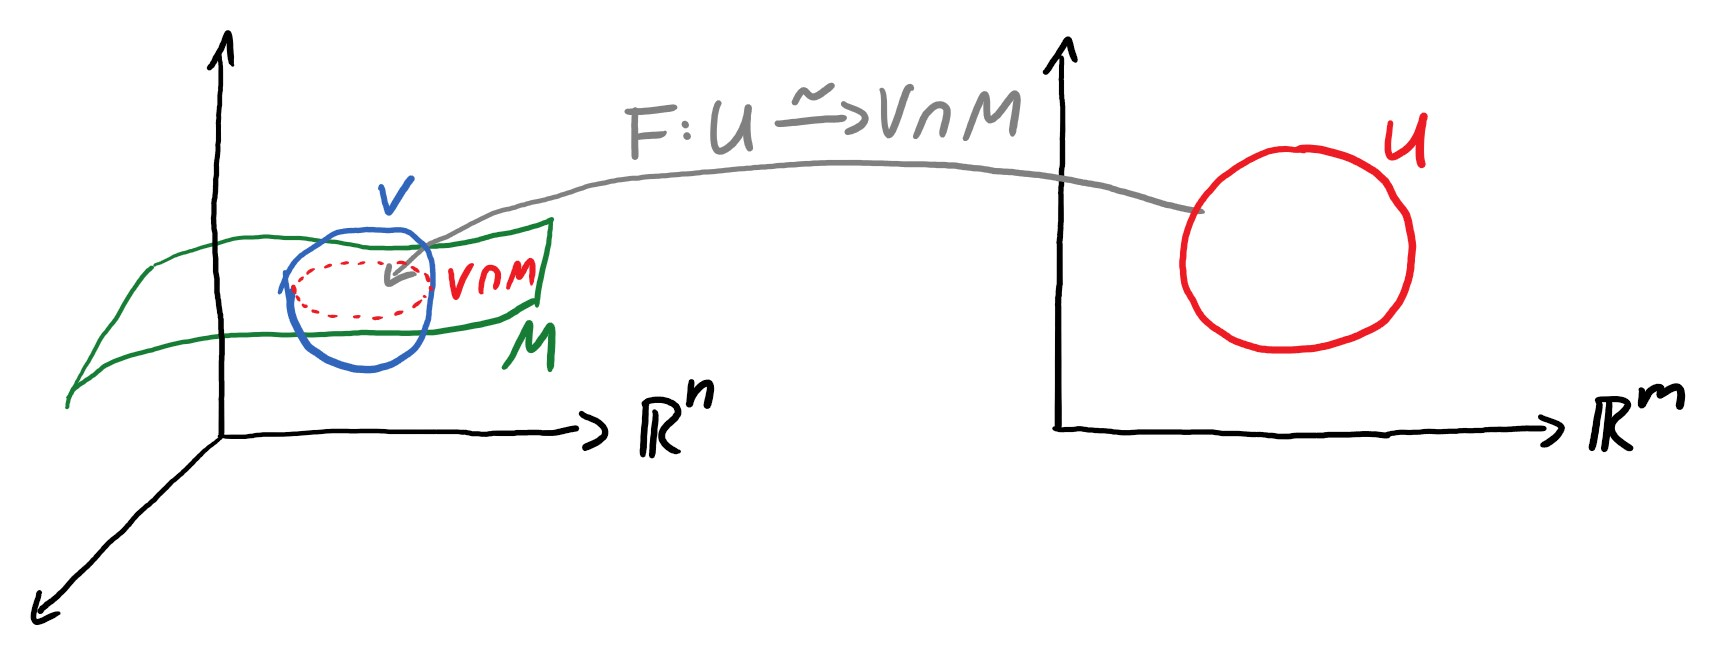
\includegraphics[width=.8\textwidth]{Dateien/10/10Untermannigfaltigkeiten.jpg}
\end{center}
\blue{Man kann dabei durchaus einen Globus im Hinterkopf haben. Lokal kann ein (dreidimensionaler) Globus immer durch eine zweidimensionale Karte (z. B. Hamburg) dargestellt werden, die sämtliche Informationen über Längen und Abstände erhält (was Homöomorphismen ja auch tun).}
\begin{Beispiel}
{Kreislinie}
Die offene Kreislinie $S^1\setminus\MengeDirekt{(1,0)}=\Menge{(x_1,x_2)\in\mathbb{R}^2\setminus\MengeDirekt{(1,0)}}{x^2_1+x_2^2=1}$ ist eine Hyperfläche des $\mathbb{R}^2$.\\
Eine mögliche Parametrisierung für alle Punkte aus dieser 1D-Untermannigfaltigkeit ist
\begin{equation*}
    F:(0,2\pi)\overset{\sim}{\to}S^1\setminus\MengeDirekt{(1,0)}, \quad F(t)=\Matrix{\cos(t)\\\sin(t)}.
\end{equation*}
\begin{center}
    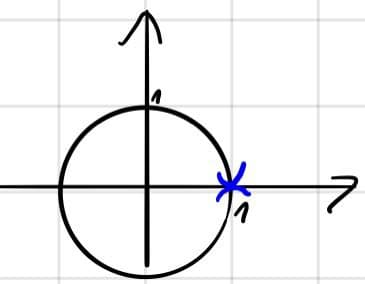
\includegraphics[width=.15\textwidth]{Dateien/10/10Kreislinie.jpg}
\end{center}
\end{Beispiel}

\begin{Def}
    {Allgemeine Mannigfaltigkeiten}
    Gegeben seien ein metrischer Raum $M$, eine offene Überdeckung $(v_i)_{i\in I}$ von $M$ mit offenen Mengen $U_i \subseteq \mathbb{R}^m$ und Homöomorphismen 
    \begin{equation*}
        F_i:\, U_i\overset{\sim}{\rightarrow} V_i.
    \end{equation*}
    Man spricht dann von einer (abstrakten) m-dimensionalen $C^k$-Mannigfaltigkeit, wenn für je zwei offene Mengen $V_1,V_2\subseteq M$ mit Abbildungen $F_1$ und $F_2$ die Abbildung
    \begin{equation*}
        F_2^{-1}\circ F_1:\, F_1^{-1}(V_1\cap V_2) \rightarrow F_2^{-1}(V_1\cap V_2)
    \end{equation*}
    ein $C^k$-Diffeomorphismus ist.
\end{Def}
\blue{Die abstrakte Mannigfaltigkeit wird in den Mathevorlesungen für euch (glücklicherweise) keine große Rolle mehr spielen. Wenn ihr euch allerdings mit allgemeiner Relativitätstheorie auseinandersetzen wollt, kommt ihr früher oder später nicht mehr an diesem Begriff vorbei. Der Vollständigkeit halber bringen wir auch hier eine Zeichnung, um das Konzept hoffentlich etwas plausibler zu machen.}
\begin{center}
    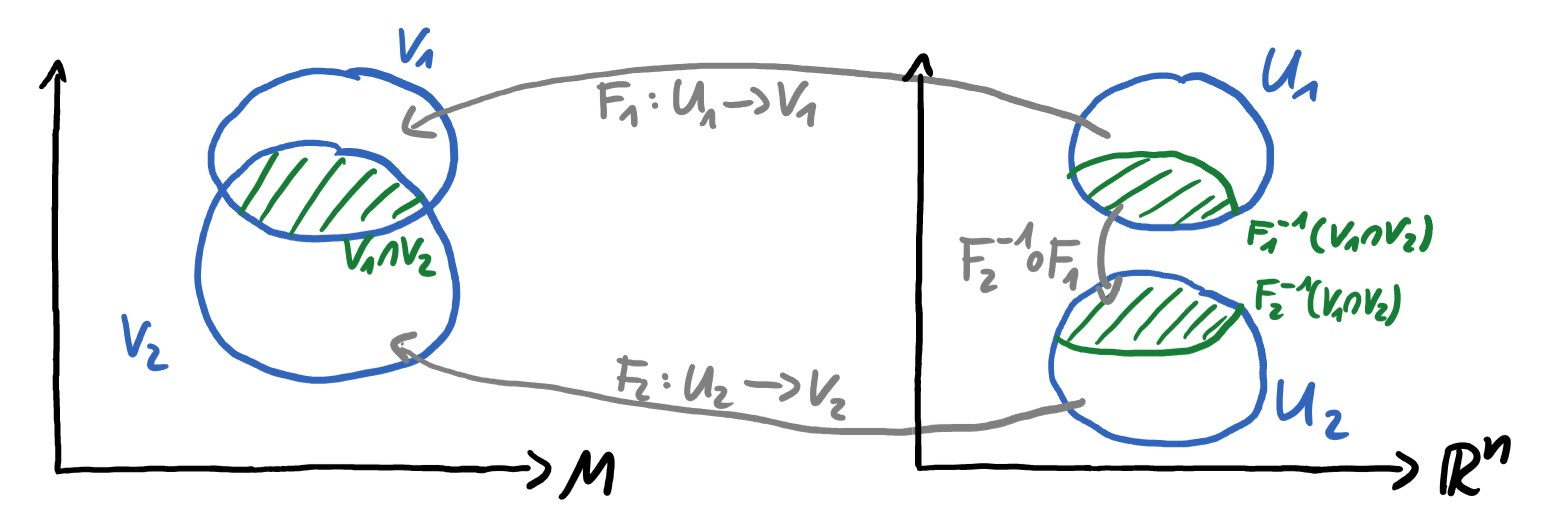
\includegraphics[width=.8\textwidth]{Dateien/10/10Mannigfaltigkeit.jpg}
\end{center}
\blue{Man beachte, dass eine Untermannigfaltigkeit stets in den $\mathbb{R}^n$ eingebettet ist, währen die Mannigfaltigkeit selbst der topologische Raum ist (also keine Einbettung besitzt). Salopp formuliert kann man auch sagen, dass eine Mannigfaltigkeit ein metrischer Raum ist, der lokal wie der $\mathbb{R}^n$ aussieht.}

\subsubsection{Parametrisierung von Untermannigfaltigkeiten}
\blue{Im Folgenden schauen wir uns die beiden im Skript genannten Möglichkeiten an, mit deren Hilfe ihr Untermannigfaltigkeiten parametrisieren könnt. \\
Der erste Satz besagt, dass man Untermannigfaltigkeiten durch Graphen von k-fach differenzierbaren Funktionen darstellen kann.}
\begin{Satz}
    {Darstellung von Untermannigfaltigkeiten als Graph}
    Eine Teilmenge $M\subseteq\mathbb{R}^n$ ist genau dann eine m-dimensionale $C^k$-Untermannigfaltigkeit, wenn es zu jedem Punkt $a\in M$, eventuell nach Umbenennung der Koordinaten des $\mathbb{R}^n$, offene Umgebungen $U'\subseteq\mathbb{R}^m$ von $a':=(a_1,...,a_m)$ und $U''\subseteq\mathbb{R}^{n-m}$ von $a'':=(a_{m+1},...,a_n)$ und eine $C^k$-Abbildung $g:U'\rightarrow U''$ gibt, sodass
    \begin{equation*}
        M\cap(U'\times U'')=\Menge{(x',x'')\in U'\times U''}{x''=g(x')}
    \end{equation*}
    gilt.
\end{Satz}
\blue{Ja, dieser Satz sieht auf den ersten Blick aus wie die Ausgeburt der Hölle, aber er enthält im Grunde zwei sehr einfache Aussagen:
\begin{enumerate}
    \item Jede Untermannigfaltigkeit lässt sich lokal als Graph einer $C^k$-Abbildung parametrisieren
    \item Umgekehrt ist der Graph jeder $C^k$-Abbildung auf einem offenen Intervall eine Untermannigfaltigkeit
\end{enumerate}
Auch die folgende Zeichung soll dabei helfen, den Satz etwas besser einordnen zu können:}
\begin{center}
    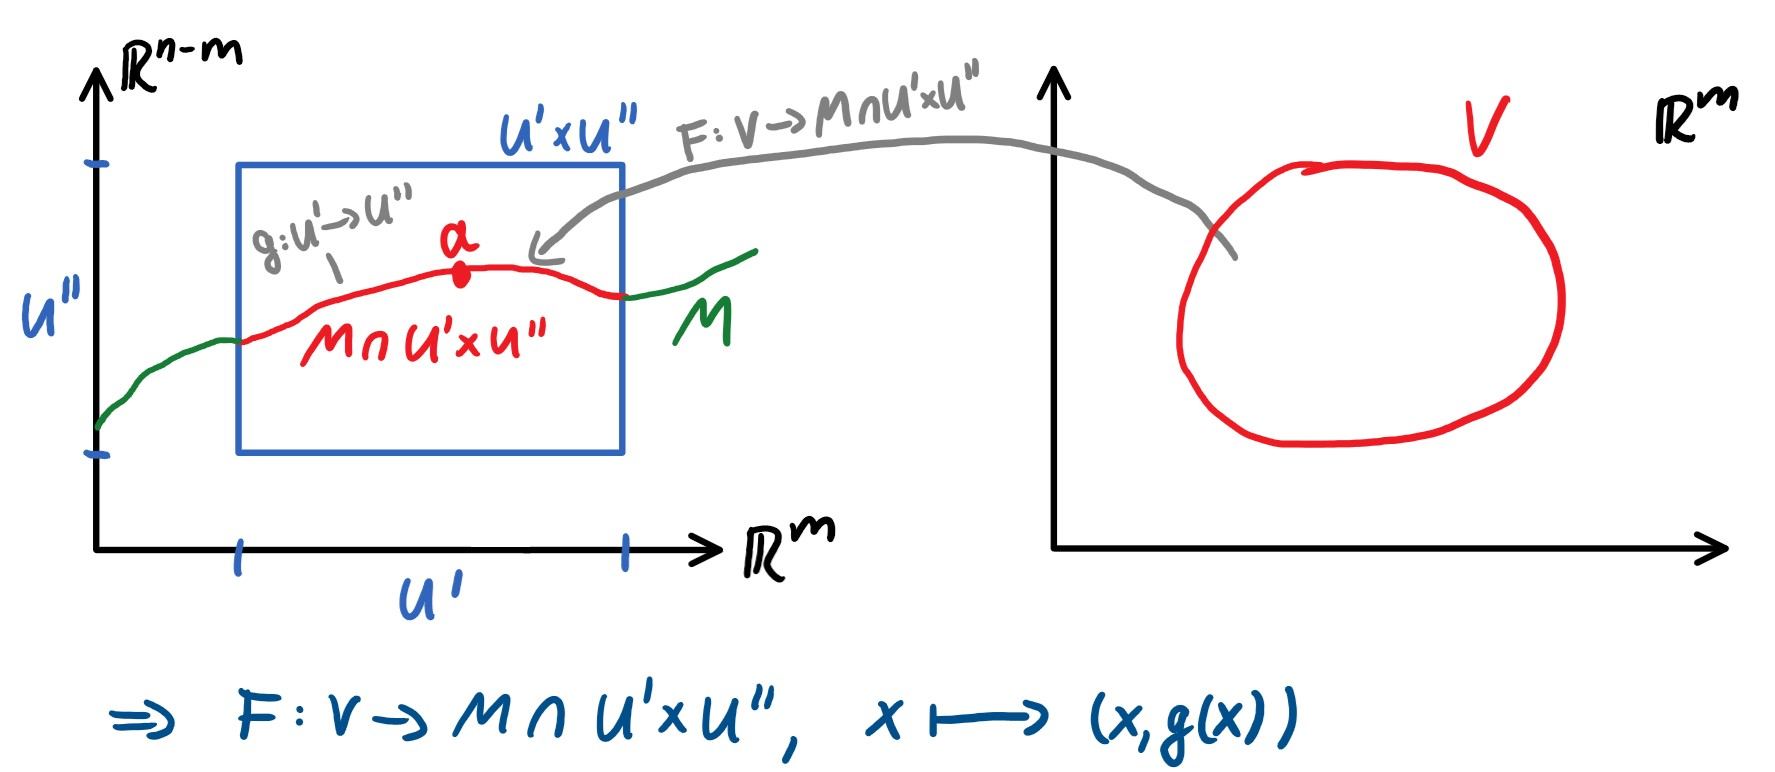
\includegraphics[width=.8\textwidth]{Dateien/10/10UntermannigfaltigkeitenAlsGraph.jpg}
\end{center}
\blue{Wichtig ist auch das folgende Beispiel:}
\begin{Beispiel}
    {Karte eines Funktionsgraphen}
    Sei $f: U\subseteq\mathbb{R}^n\rightarrow\mathbb{R}$ eine $C^k$-Funktion mit $k\geq 1$. Dann ist $F:U\subseteq\mathbb{R}^n\rightarrow\mathbb{R}^{n+1}, F(x)=(x,f(x))$ eine Immersion, denn
    \begin{equation*}
        \text{d}F_x=\Matrix{1 & \ldots & 0 \\ \vdots & \ddots & \vdots \\ 0 & \ldots & 1 \\ \partial_1 f(x) & \ldots & \partial_n f(x)} \quad \Rightarrow \quad \text{rg}(\text{d}F_x) = n
    \end{equation*}
    hat konstanten Rang $n$. Das Bild von $F$ ist der Graph $\Gamma_f$ von $f$. \\
    Es gibt offensichtlich eine Umkehrfunktion $F^{-1}:\,\Gamma_f\rightarrow\mathbb{R}\quad(x,f(x))\mapsto x$. Sowohl $F$ als auch $F^{-1}$ sind per Definition von $f$ stetig, sodass $F$ ein waschechter Homöomorphismus ist.
\end{Beispiel}
\begin{Beispiel}
    {Stereographische Projektion Reloaded}
    Wir betrachten wieder die stereographische Projektion. Den oberen Halbkreis können wir durch den Graphen der folgenden Funktion parametrisieren:
    \begin{equation*}
        f(x)=\sqrt{r^2-x^2} \quad r\in\mathbb{R}.
    \end{equation*}
    Dies ist eine $C^\infty$-Abbildung. Besagter Graph ist dann
    \begin{equation*}
        \Gamma_f=\Menge{(x,f(x))\in\mathbb{R}^2}{x\in(-r,r)}.
    \end{equation*}
    Eine einfache Karte dieser Untermannigfaltigkeit wäre gegeben durch
    \begin{equation*}
        F:(-r,r)\rightarrow\Gamma_f, \quad F(x)=(x,\sqrt{r^2-x^2}).
    \end{equation*}
    Dies ist aber nicht die einzige Möglichkeit, wie wir bereits gesehen haben. Auch die stereographische Projektion ist eine mögliche Karte.
    \begin{equation*}
        \varphi:\,\mathbb{R}\setminus[-r,r]\longrightarrow \Gamma_f, \quad \varphi(x)=\frac{r}{x^2+r^2}(2rx, x^2-r^2)
    \end{equation*}
\end{Beispiel}


\blue{Jetzt kommen wir zur zweiten Möglichkeit, nämlich der Parametrisierung von Untermannigfaltigkeiten als Urbilder unter Abbildung von konstantem Rang.}
\begin{Satz}
{Satz}{Untermannigfaltigkeiten als Urbilder unter Abbildungen von konstantem Rang}
Sei $U\subseteq\mathbb{R}^n$ offen und $f:U\to\mathbb{R}^m$.
\begin{itemize}
    \item Ist $f$ eine $C^k$-Abbildung,
    \item hat $f$ konstanten Rang $r$ und
    \item ist $\qvec\in f(U)$,
\end{itemize}
so ist das Urbild\footnote{also alle Punkte, die auf $\qvec$ abgebildet werden} des Punktes $\qvec$ eine $C^k$-Untermannigfaltigkeit des $\mathbb{R}^n$ der Dimension \red{m=n-r}, also
\begin{equation}
    M:=f^{-1}(\qvec)\subseteq U.
\end{equation}
\begin{center}
    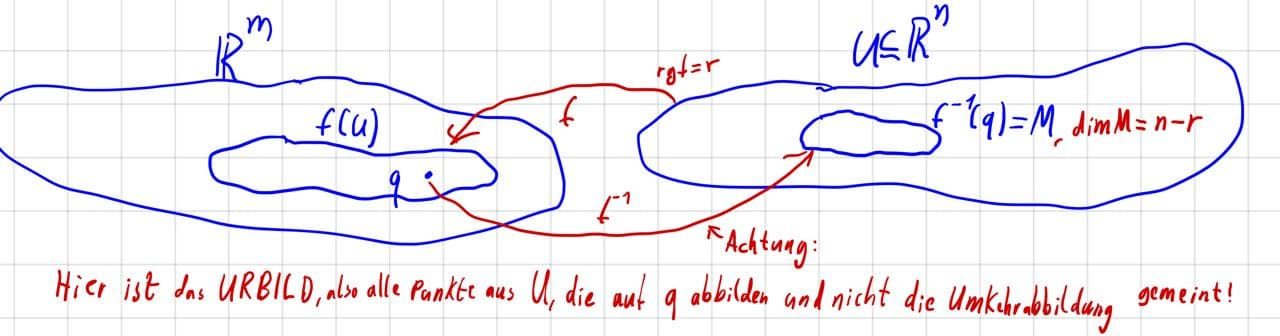
\includegraphics[width=.5\textwidth]{Dateien/10/10UMF1.jpg}
\end{center}
\end{Satz}
\blue{Quasi als Umkehrung dieses Satzes hattet ihr auch die folgende Aussage:}
\begin{Satz}
{Satz}{Untermannigfaltigkeiten und Submersionen}
$M\subseteq \mathbb{R}^n$ ist genau dann eine $m$-dimensionale Untermannigfaltigkeit, \\
wenn es für alle $\pvec\in M$ eine Umgebung $V\subseteq \mathbb{R}^n$ von $\pvec$ und eine Submersion\footnote{Abbildung mit konstantem Rang $n-m$} $f:V\to\mathbb{R}^{n-m}$ mit $f^{-1}(0)=M\cap V$ gibt.
\begin{center}
    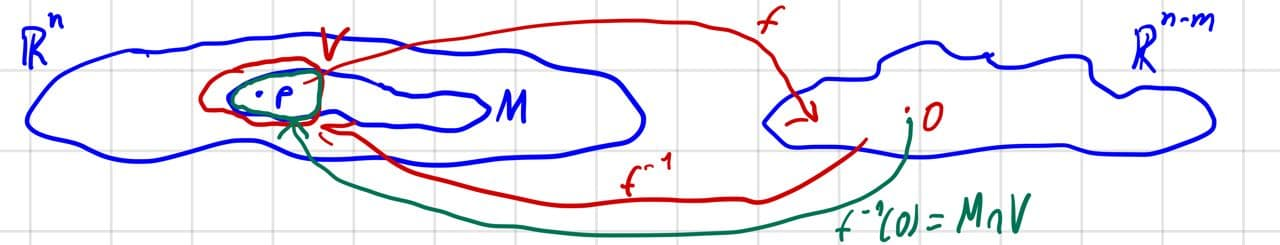
\includegraphics[width=.5\textwidth]{Dateien/10/10UMF2.jpg}
\end{center}
\end{Satz}
blue{Diese besagt, dass $M$ also in der Umgebung $V$ um $\pvec\in M$ durch ein Gleichungssystem mit $n-m$ Gleichungen beschrieben werden kann ($f^{-1}(0)=M\cap V$).} \\

blue{Die zentralen Aussagen dieser beiden Sätze sind:
\begin{enumerate}
    \item Jede Untermannigfaltigkeit lässt sich lokal durch das Urbild eines Punktes unter einer $C^k$-Submersion parametrisieren.
    \item Durch das Urbild eines Punktes unter einer $C^k$-Submersion ist immer eine Untermannigfaltigkeit definiert
\end{enumerate}
Jetzt kommen wir wieder zu ein paar Beispielen.}

\begin{Beispiel}
    {Die Kugel (1/2)}
    Gegeben ist die Funktion $f:\mathbb{R}^3\rightarrow\mathbb{R},\quad f(x,y,z)=x^2+y^2+z^2$ und ein Punkt $a\in\mathbb{R_+}\setminus\{0\}$. \\
    Wir Behaupten: Das Urbild $f^{-1}(a)$ ist eine $C^\infty$-Untermannigfaltigkeit des $\mathbb{R}^3$ der Dimension 2. \\
    Für den Beweis benutzen wir einfach den Satz über Untermannigfaltigkeiten als Urbilder unter Abbildungen von konstantem Rang. Dafür stellen wir fest:
    \begin{itemize}
        \item $f(x,y,z)$ ist $\infty$-oft differenzierbar
        \item Das Differential ist
        \begin{align*}
            \text{d}f=\Matrix{\partial_1 f & \partial_2 f & \partial_3 f} = \Matrix{2x & 2y & 2z} \\
            \Rightarrow \text{rg}(f)=\text{rg}(\text{d}f)=1 \quad \forall(x,y,z)\in f^{-1}(a)
        \end{align*}
        also ist $f$ eine Abbildung von konstantem Rang.
    \end{itemize}
    Weiterhin müssen wir noch sicherstellen, dass alle Punkte $\mathbb{R}\setminus\{0\}$ tatsächlich im Bild von $f$ liegen (dieser Schritt ist nicht bei allen Aufgaben dieser Art nötig). Dies ist aber ganz einfach, denn 
    \begin{equation*}
        f(0,\mathbb{R}_+,0)=\mathbb{R}_+,
    \end{equation*}
    da für jede Zahl $x\in\mathbb{R}_+$ eine Zahl $y\in\mathbb{R}_+$ existiert, sodass $y^2=x$. Es gilt also $a\in\mathbb{R_+}\setminus\{0\}\subseteq f(\mathbb{R}^3)$. \\
    Mit diesen Erkenntnissen folgt die Aussage direkt aus dem entsprechenden Satz. Die Dimension der Untermannigfaltigkeit ist $3-1=2$. \\
    
    Wir setzen nun $a=1$ und suchen eine Parametrisierung einer Umgebung des Punktes $(0,0,1)$ in $f^{-1}(1)$. Dazu betrachten wir die Gleichung
    \begin{equation*}
        f(x,y,z)=x^2+y^2+z^2=1
    \end{equation*}
    und stellen nach $z$ um (wobei man genauso gut nach $x$ oder $y$ umstellen kann, das ist am Ende Geschmackssache)
    \begin{equation*}
        z_\pm = \pm \sqrt{1-x^2-y^2}.
    \end{equation*}
    Wir untersuchen explizit die Umgebung des Punktes $(0,0,1)$, also ist die gesuchte Lösung
    \begin{equation*}
        z_+=\sqrt{1-x^2-y^2}
    \end{equation*}
    und wir können die Punkte in der Umgebung durch den Graphen von $z_+$ parametrisieren durch
    \begin{equation*}
        \Gamma_{z_+} := \Menge{(x,y,z)\in\mathbb{R}^3}{z=\sqrt{1-x^2-y^2}}.
    \end{equation*}
    Dies ist die obere Hemisphäre der Kugel. Die untere Hemisphäre wird durch den Graphen von $z_-$ parametrisiert. Die Karte können wir nun wie üblich wie folgt hinschreiben:
    \begin{equation*}
        F: \mathbb{R}^2\rightarrow\Gamma_f, \quad F(x,y)=(x,y,\sqrt{1-x^2-y^2}).
    \end{equation*}
\end{Beispiel}
\begin{Beispiel}
    {Und noch ein Beispiel (2/2)}
    Gegeben sind die beiden Funktionen
    \begin{equation*}
        f_1(x)=x_1^2+x_1x_2-x_2-x_3 \qquad f_2(x)=x_1^2+3x_1x_2-2x_2-3x_3
    \end{equation*}
    und die Menge
    \begin{equation*}
        C:=\Menge{x\in\mathbb{R}^3}{f_1(x)=f_2(x)=0}.
    \end{equation*}
    Wir behaupten nun, dass $C$ eine eindimensionale $C^{\infty}$-Untermannigfaltigkeit des $\mathbb{R}^3$ ist. Dazu betrachten wir die Funktion $f:\mathbb{R}^3\rightarrow\mathbb{R}^2$, gegeben durch
    \begin{equation*}
        f(x)=\Matrix{f_1(x) \\ f_2(x)}
    \end{equation*}
    und stellen fest:
    \begin{itemize}
        \item $f$ ist $\infty$-oft differenzierbar
        \item Das Differential ist
        \begin{align*}
            \text{d}f&=\Matrix{2x_1+x_2 & x_1-1 & -1 \\ 4x_1+3x_2 & 3x_1-2 & -3} \overset{Gauß}{\longrightarrow} \Matrix{2x_1 & x_1-1 & -1 \\ -2x_1 & -1 & 0} \\
            &\Rightarrow \text{rg}(f)=\text{rg}(\text{d}f)=2 \quad \forall x\in\mathbb{R}^3
        \end{align*}
        also ist $f$ eine Abbildung von konstantem Rang..
    \end{itemize}
    Die Behauptung folgt dann wieder direkt aus dem Satz über Untermannigfaltigkeiten als Urbilder unter Abbildungen von konstantem Rang. Die Untermannigfaltigkeit hat demnach auch die behauptete Dimension $3-2=1$.
\end{Beispiel}

\begin{Def}
{Tangentialvektoren und Tangentialraum}
Für eine $C^1$-Untermannigfaltigkeit $M\subseteq\mathbb{R}^n$ nennen wir für einen Punkt $\pvec\in M$ gelegte Vektoren $\vvec\in\mathbb{R}^n$ \red{Tangentialvektoren}, wenn
\begin{itemize}
    \item ...es $\epsilon>0$ und eine stetig differenzierbare Kurve $\gamma:(-\epsilon,\epsilon)\to M$ gibt, welche
    \begin{itemize}
        \item durch den Punkt $\pvec$ verläuft, also $\gamma(0)=\pvec$ und
        \item für die $\vvec=\gamma'(0)$ gilt.
    \end{itemize}
\end{itemize}
Die Menge aller Tangentialvektoren an die UMF $M$ im Punkt $\pvec$ nennen wir \red{Tangentialraum} in $\pvec$.\\
Wir schreiben auch $T_\pvec M$.
\end{Def}
\begin{Satz}
{Satz}{Eigenschaften des Tangentialraums}
Für den Tangentialraum $T_\pvec M$ an einer UMF $M$ im Punkt $\pvec$ gilt:
\begin{itemize}
    \item $T_\pvec M$ ist ein Vektorraum mit $\dim (T_\pvec M)=m=\dim M$.
    \item Falls wir mit $F:U\to V$ eine lokale Parametrisierung von $M$ haben, sodass $F(\uvec)=\pvec$ ist ($\uvec\in U$),\\
    dann bilden die Vektoren $\partial_1F(\uvec),\ldots,\partial_mF(\uvec)$ eine Basis des Tangentialraums.
\end{itemize}
\end{Satz}
Den Tangentialraum können wir uns für einen Punkt $\pvec$ an einer Kugel $M$ als Ebene vorstellen, die an diesen Punkt angelegt wird.\\
Er ist später in der Differentialgeometrie von Bedeutung, an dieser Stelle betrachten wir ihn vor allem, um ihn im folgenden Satz nutzen zu können.

\subsection{Lagrange-Multiplikatoren}
\blue{Der folgende Satz hilft uns bei mehrdimensionalen Optimierungsaufgaben, bei denen wir Extrema von Mengen unter bestimmten Nebenbedingungen zu finden versuchen.\\
Ein klassisches Beispiel ist die Bestimmung minimaler Abstände zwischen geometrischen Objekten.\\
In der äquivalenten Formulierung (s. u.) ist er deutlich leichter zu verstehen.}
\begin{Satz}
{Satz}{Extrema mit Nebenbedingungen}
Wir betrachten eine \red{m}-dimensionale Untermannigfaltigkeit $M\subseteq\mathbb{R}^{\red{n}}$ des $\mathbb{R}^n$ und eine Funktion $f:U\to\mathbb{R}$ (wobei $U\subseteq\mathbb{R}^n$), die im Punkt $\pvec\in M\cap U$, d. h. auf der Untermannigfaltigkeit, differenzierbar ist.\\
Nimmt die Funktion $f$ eingeschränkt auf die Untermannigfaltigkeit $U\cap M$ im Punkt $\pvec$ ein \underline{lokales Extremum} an, so gilt
\begin{equation*}
    T_\pvec M\subseteq\ker(df_\pvec)=(\grad(f(\pvec)))^\perp,
\end{equation*}
in Worten:\\
Der Tangentialraum\footnote{welcher, wie eben gesehen, alle Vektoren beinhaltet, die im Punkt $\pvec$ tangential auf der Untermannigfaltigkeit liegen}, den wir an den Punkt $\pvec$ bzgl. $M$ anlegen, ist eine Teilmenge des Kerns des Differentials von $f$ in $\pvec$ (also jener Vektoren $\xvec\in\mathbb{R}^n$ mit $df_\pvec\cdot\xvec=0$.\\
Dieser Kern entspricht genau dem orthogonalen Komplement von $\grad (f(\pvec))$.
\begin{center}
    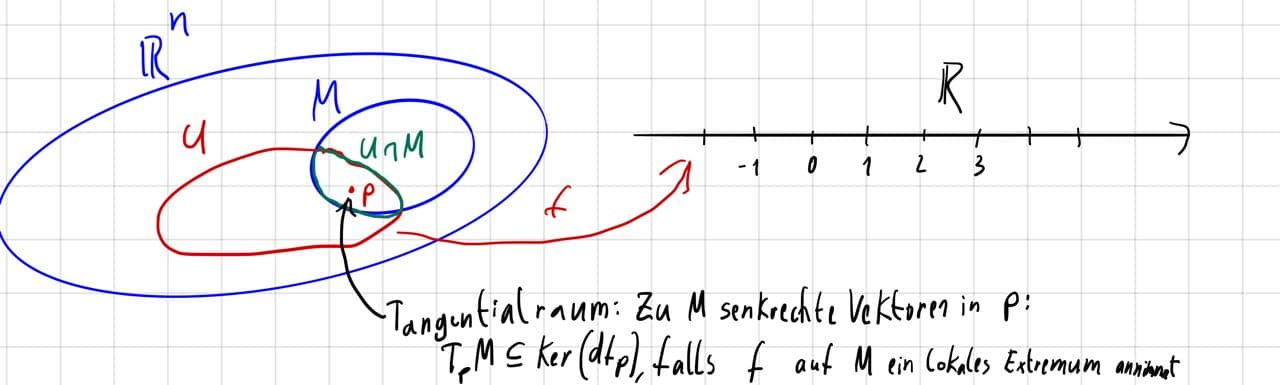
\includegraphics[width=.5\textwidth]{Dateien/10/10Lagrange1.jpg}
\end{center}
\end{Satz}
\begin{Satz}
{Satz}{Äquivalente Formulierung mit Lagrange-Multiplikatoren}
Ebenso können wir sagen:\\
Nimmt $f$ auf $M$ ein lokales Extremum im Punkt $\pvec$ an, so folgt, dass\\
Konstanten $\boxed{\lambda_1,\ldots,\lambda_{\red{r}}\in\mathbb{R}}$ (auch \red{Lagrange-Multiplikatoren} genannt) existieren, sodass das Gleichungssystem
\begin{equation*}
    \grad(f(\pvec))=\sum_{j=1}^{\red{r}}\lambda_i\grad(h_j(\pvec))
\end{equation*}
erfüllt ist.\\
Hierzu benötigen wir zusätzlich die Abbildung $h:U\to\mathbb{R}^r$, für die $M\cap U$ das Urbild des Nullvektors sein muss, d. h. $h^{-1}(0)=M\cap U$. $h$ muss eine \underline{stetig differenzierbare Submersion} (d. h. mit konstantem Rang $\rg(h)=r=n-m$) sein.
\end{Satz}

\begin{Beispiel}
{Extrema unter Nebenbedingungen (1/2)}
Wir suchen
\begin{equation*}
    \min\Menge{x-y,\, (x,y)\in\mathbb{R}^2\setminus\MengeDirekt{(0,2)}}{x^2+(y-2)^2=1}.
\end{equation*}
\begin{itemize}
    \item Mit der Kreislinie $x^2+(y-2)^2=1$ liegt eine $m=n-r=2-1=1$-dimensionale Untermannigfaltigkeit im $\mathbb{R}^{n=2}$ vor\footnote{Dies folgt aus dem Satz über Untermannigfaltigkeiten als Urbilder von Abbildungen von konstantem Rang}.
    \item Die zu minimierende Funktion\footnote{aufgrund der Nebenbedingung kann man erkennen, dass sie nicht nur durch \underline{eine} Gleichung beschrieben wird.} $\boxed{f(x,y)=x-y}$ entspricht $f:\mathbb{R}^2\to\mathbb{R}$.
    \item Die Funktion $h(x,y)=x^2+(y-2)^2-1$ entspricht $h:\mathbb{R}^2\to\mathbb{R}^{r=1=2-1=n-m}$, denn es gilt $h^{-1}(0)=M\cap\mathbb{R}^2$ und $h$ ist eine stetig differenzierbare Submersion auf $h^{-1}(0)$, da $dh=\MatrixInline{2x& 2(y-2)}$ auf $\mathbb{R}^2\setminus\MengeDirekt{(0,2)}$ konstanten Rang 1 hat.
\end{itemize}
Daher ist der Satz anwendbar.\\
$M=h^{-1}(0)$ ist also eine Untermannigfaltigkeit der Dimension 1.\\
Angenommen, $(x_0, y_0)\in M$ minimiert $f(x,y)$, so muss $\lambda$\footnote{nur ein $\lambda$, weil $r=1$ ist} existieren, sodass
\begin{equation*}
    \grad(f(x_0,y_0))=\lambda\grad(h(x_0,y_0)).
\end{equation*}
Dies sind also zwei bestimmende Gleichungen:
\begin{align*}
    1&=\lambda 2x_0\quad \tx{(aus }\partial_xf\big|_{(x_0,y_0)}=\lambda\partial_xh\big|_{(x_0,y_0)})\\
    -1&=\lambda 2(y_0-2)\quad \tx{(aus }\partial_yf\big|_{(x_0,y_0)}=\lambda\partial_yh\big|_{(x_0,y_0)})\\
    0&=x_0^2+(y_0-2)^2-1\quad \tx{(aus der Bedingung }h^{-1}(0)=M)
\end{align*}
Formen wir dies um, so sehen wir:\\
1. Gleichung: $x_0=\frac{1}{2\lambda}$\\
2. Gleichung: $y_0=-\frac{1}{\lambda^2}+2$\\
Einsetzen in 3: $\frac{1}{4\lambda^2}+\frac{1}{4\lambda^2}=1\iff \lambda_\pm=\pm\frac{1}{\sqrt{2}}$\\
Damit haben wir
\begin{align*}
    \lambda_+:\quad x_0&=\frac{\sqrt{2}}{2},\quad y_0=\frac{-\sqrt{2}}{2}+2,\\
    \lambda_-:\quad x_0&=-\frac{1}{\sqrt{2}},\quad y_0=\frac{1}{\sqrt{2}}+2.
\end{align*}
Die Punkte $\pvec_1=\MatrixInline{1/\sqrt{2}\\2-1/\sqrt{2}}$ und $\pvec_2=\MatrixInline{-1/\sqrt{2}\\2+1/\sqrt{2}}$ maximieren und minimieren also $f$ mit $f(\pvec_1)=x_1-y_1=\sqrt{2}-2$ und $f(\pvec_2)=-\sqrt{2}-2$.\\
Bisher haben wir also gezeigt, dass für $\pvec_2$ das \red{notwendige Kriterium} für ein Minimum erfüllt ist.
\begin{center}
    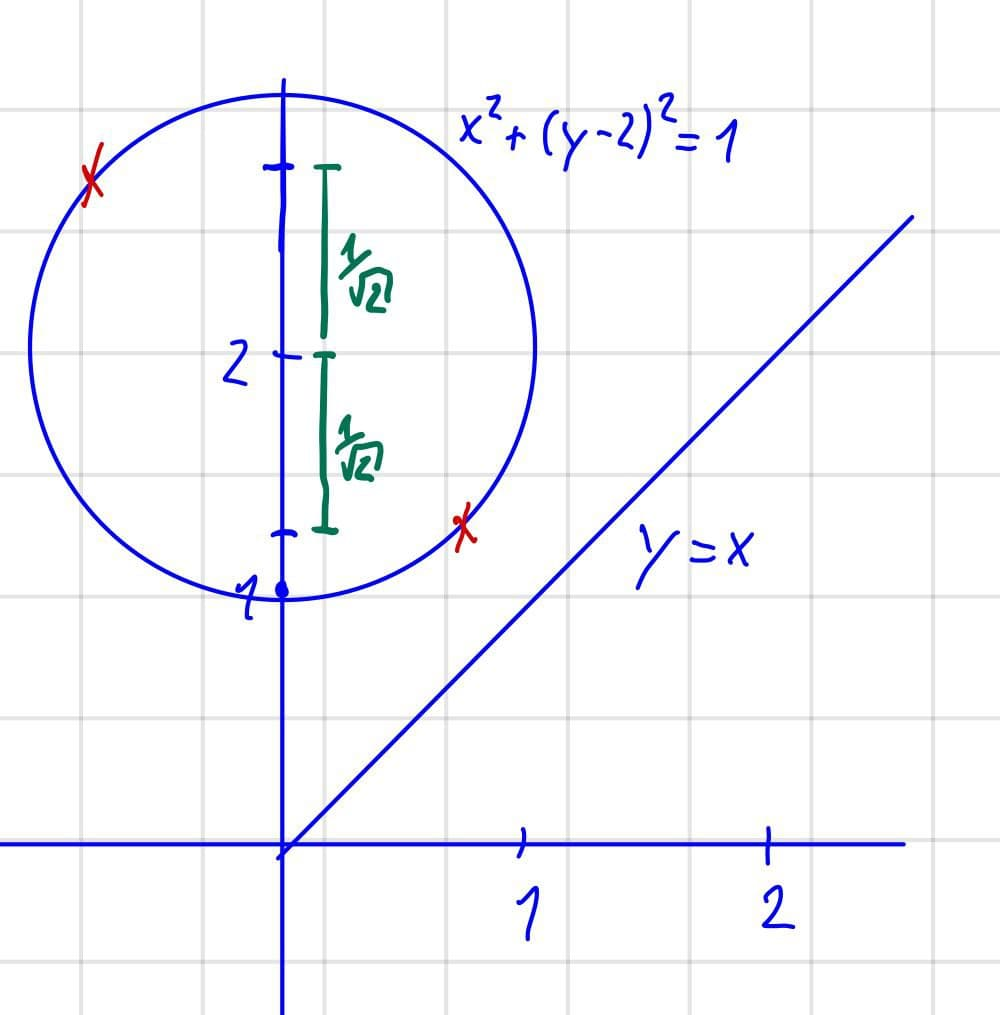
\includegraphics[width=.25\textwidth]{Dateien/10/10LagrangeBild.jpg}
\end{center}
Anschauung: Beim linken Punkt ist $x-y$ minimal, beim rechten ist $x-y$ maximal.
Warum muss das aber nun ein Extremum sein?\\
Die Mannigfaltigkeit $M$ ist nach dem Satz von Heine-Borel kompakt, da sie eine abgeschlossen (das Komplement auf $\mathbb{R}^2$ ist offen) und beschränkte Teilmenge des $\mathbb{R}^2$ ist, wie man z. B. durch folgende Abschätzung sehen kann:
\begin{equation*}
    \xvec\in M:\, \Norm{\xvec}^2=x^2+y^2\overset{\footnote{$(y-2)^2=1-x^2\iff y-2=\pm\sqrt{1-x}\iff y^2=\BracedIn{2\pm\sqrt{1-x^2}}^2.$ Zudem sieht man hier, dass $x\in[-1,1]$ sein muss.}}{=}x^2+4\pm 4\sqrt{1-x^2}+1-x^2=5\pm\sqrt{1-x^2}\leq 5+4.
\end{equation*}
Als stetige Funktion, die auf einem Kompaktum $M$ definiert ist, muss $f$ Minimum und Maximum annehmen.\\
Da die einzigen dafür in Frage kommenden Punkte mithilfe der Methode der Lagrange-Multiplikatoren gefunden wurden und quasi alle Punkte von vornherein auf dem Rand der Menge liegen, handelt es sich bei $\pvec_2$ also um ein Minimum.\\
\blue{Die Argumentation ist also: Weil eine kompakte Menge vorliegt, $f$ stetig ist und die Punkte bereits auf dem Rand liegen, muss es sich um ein globales Minimum handeln.}
\end{Beispiel}

Bei unbeschränkten UMF muss man sich eines weiteren Tricks bedienen:
\begin{Beispiel}
{Weitere Extrema unter Nebenbedingungen (2/2)}
Wir suchen
\begin{equation*}
    \max\Menge{xy+yz+xz,\, (x,y,z)\in\mathbb{R}^3}{x+y+z=120}.
\end{equation*}
\begin{itemize}
    \item Hier ist $h:\mathbb{R}^{n=3}\to\mathbb{R}^{r=1}h(x,y,z)=x+y+z-120$, was eine stetig differenzierbare Submersion ist, da $\rg(h)=\rg(dh)=\rg\MatrixInline{1&1&1}=1=r$ ist.
    \item $M:=h^{-1}(0)$ ist als Urbild unter einer Abbildung von konstantem Rang 1 eine Untermannigfaltigkeit der Dimension $m=\dim M=n-r=3-1=2$.
    \item Zudem ist $f(x,y,z)=xy+yz+xz$ die gewünschte Funktion $f:\mathbb{R}^3\to\mathbb{R}$, die maximiert werden soll.
\end{itemize}
Der Satz ist also anwendbar, wir können folgern:\\
Ist $\pvec=(x_0,y_0,z_0)$ ein Extremum, so existiert $\lambda$\footnote{wieder nur ein $\lambda$, da $r=1$}, sodass $\grad(f(\pvec))=\lambda\grad(h(\pvec))$. Also haben wir die Gleichungen
\begin{equation*}
    y_0+z_0=\lambda,\quad x_0+z_0=\lambda,\quad x_0+y_0=\lambda,
\end{equation*}
woraus wir $z_0=x_0=y_0=\frac{\lambda}{2}$ folgern können.\\
Zusätzlich (weil $\pvec\in M$ sein muss) wissen wir, dass
\begin{equation*}
    x_0+y_0+z_0-120=0\implies 3\frac{\lambda}{2}=120\implies \lambda=80\implies x_0=y_0=z_0=40.
\end{equation*}
Nun ist noch zu zeigen, dass $\pvec=(40,40,40)$ tatsächlich ein Maximum ist:\\
$h(40,40,40)=4800$ ist also der eventuell maximale Wert.\\
Wie im ersten Beispiel definieren wir uns als Trick nun eine kompakte Menge:\\
Sei $N=M\cap P=M\cap\Menge{(x,y,z)\in\mathbb{R}^3}{xy+yz+xz\leq4800}$. Dies ist eine abgeschlossene, beschränkte TM des $\mathbb{R}^3$ und somit kompakt. Jede stetige Funktion nimmt auf einer kompakten Menge ihr Minimum und Maximum an.\\
Der einzige Punkt, der hierbei als Maximum in Frage kommt, ist der gefundene Randpunkt $\pvec$. Dieser ist ein globales Maximum, da Punkte mit $xy+yz+zx>4800$ nicht mehr auf $M$ liegen.
\end{Beispiel}